\chapter{GRAMMAR PRESENTATION}
Domain-Specific Languages (DSLs) can be used to simplify the process of writing unit tests by providing a custom syntax that is tailored to the needs of the software being tested. It will introduced a grammar for a DSL that can be used for unit testing, exploring its syntax and capabilities, and demonstrating how it can be used to write effective and efficient unit tests \cite{dadario}.

It will first be introduced a bunch of examples that show how the DSL will work for some base cases. Then it will be presented the grammar that is used to parse the presented code.
In the Figure 1 it can found some examples that are already possible to be parsed in the DSL:

{ \centering 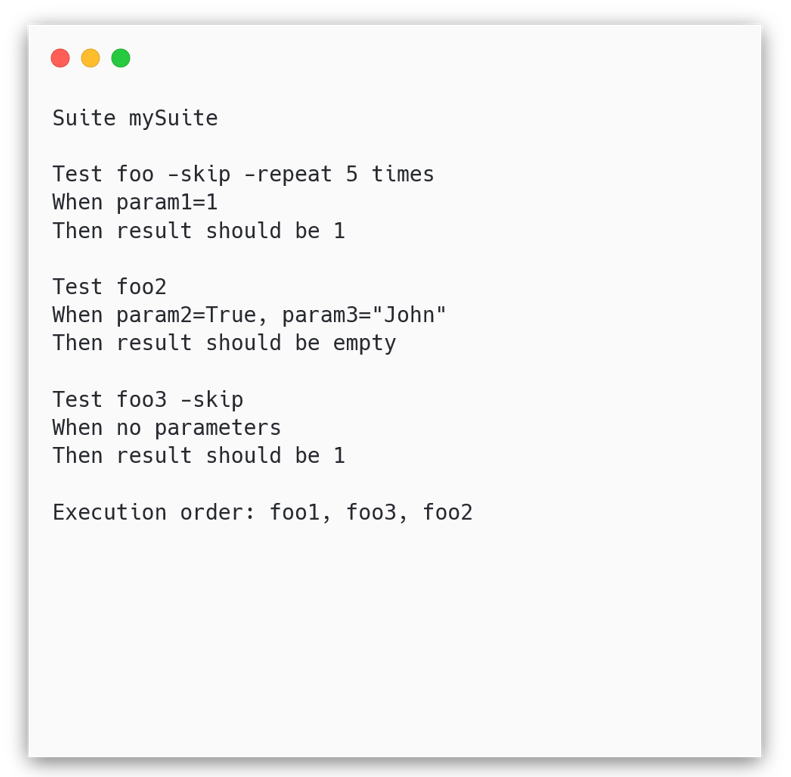
\includegraphics[width=\textwidth , height=13cm]{images/code_ex.png} }
\begin{center} Figure 1: DSL code examples \end{center}


First notice the Suite keyword. A suite defines a collection of functions. This DSL is for the Python programming language. It will search for the file that contains the name of the suite. It will then search for functions in this file.

A test is defined as follows:
Test functionName [flags]

Notice that Test is bolded, meaning it is a keyword. Following is an identifier of a function. The interpreter will search the function in the file specified in the suite definition. This function will be tested in this test. Next, optionally, flags can be specified. It was thought of the flags for skipping a test (-test), for repeating a test multiple times (-repeat N times). 

After specifying a test’s name and flags, there is the When [params]. This is the line that specifies the parameters of the function that will be called. Parameters are specified as paramName=paramValue. Notice that if a function doesn’t require (or accepts) no parameters at all, then you can just type no parameters and the function will be called without any parameters.

The last part that defines a test is the Then result should be [value]. It specifies the expected return value of the function call. Notice that a no return value (void function) also works. It is needed to type empty to mention that no value should be returned.

The keyword empty when specifying the result value is interchangeable with Empty, void, Void, none and None. Similarly, the no parameters is interchangeable with None, none, Void and void.

Lastly, it can specified the execution order of your tests. This is done by typing Execution order: [functionName1], [functionName2] and so on.

The following is a formal definition of the grammar in Backus-Naur Form (BNF):
\begin{verbatim}
VT  = {
		<letter>,
		<digit>,
		<STRING>
		<BOOL>,
		<EmptyParameters>,
		<EmptyResult>		
},

VN = {
		<ID>, <INT>, <FLOAT>, <NUMBER>,
		<Suite>, <Test>, <Result>, <Parameter>,
<Datatype>, <Flag>, <Repeat>, <Order>
}

<letter> ::= "A" | "B" | ... | "Z" | "a" | "b" | ... | "z"
<digit> ::= "0" | "1" | ... | "9"
<ID> ::= <letter> (<letter> | <digit>)*
<STRING> ::= '"' (~'"')* '"'
<INT> ::= <digit>+
<FLOAT> ::= <digit>+ "." <digit>+
<NUMBER> ::= <INT> | <FLOAT>
<BOOL> ::= "True" | "False"
<Suite> ::= "Suite" <ID> <Test>* <Order>?
<Test> ::= "Test" <ID> <Flag>* "When" <Parameter>+ <Result>
<Result> ::= "Then" ("result" "should" "be")? (<Datatype> | <EmptyResult>)
<Parameter> ::= (<ID> "=" <Datatype>) | <EmptyParameters>
<Datatype> ::= <STRING> | <INT> | <FLOAT> | <NUMBER> | <BOOL>
<EmptyParameters> ::= "no parameters" | "None" | "none" | "void" | "Void"
<EmptyResult> ::= "empty" | "Empty" | "void" | "Void" | "none" | "None"
<Flag> ::= "-" ("skip" | "Skip" | <Repeat>)?
<Repeat> ::= ("repeat" | "Repeat") <INT> ("times" | "Times")
<Order> ::= "Execution order:" <ID> ("," <ID>)*
\end{verbatim}

The language is defined as follows:
\begin{verbatim}
L(G) = (VN, VT, P, S), where
S = { <Suite> },
P = {
		<letter> => "A" | "B" | ... | "Z" | "a" | "b" | ... | "z"
<digit> => "0" | "1" | ... | "9"
<ID> => <letter> (<letter> | <digit>)*
<STRING> => '"' (~'"')* '"'
<INT> => <digit>+
<FLOAT> => <digit>+ "." <digit>+
<NUMBER> => <INT> | <FLOAT>
<BOOL> => "True" | "False"
<Suite> => "Suite" <ID> <Test>* <Order>?
<Test> => "Test" <ID> <Flag>* "When" <Parameter>+ <Result>
<Result> => "Then" ("result" "should" "be")? (<Datatype> | <EmptyResult>)
<Parameter> => (<ID> "=" <Datatype>) | <EmptyParameters>
<Datatype> => <STRING> | <INT> | <FLOAT> | <NUMBER> | <BOOL>
<EmptyParameters> => "no parameters" | "None" | "none" | "void" | "Void"
<EmptyResult> => "empty" | "Empty" | "void" | "Void" | "none" | "None"
<Flag> => "-" ("skip" | "Skip" | <Repeat>)?
<Repeat> => ("repeat" | "Repeat") <INT> ("times" | "Times")
<Order> => "Execution order:" <ID> ("," <ID>)*
}
\end{verbatim}

In Figure 2 it is represented the meta-model for the language as generated by TextX.

{ \centering 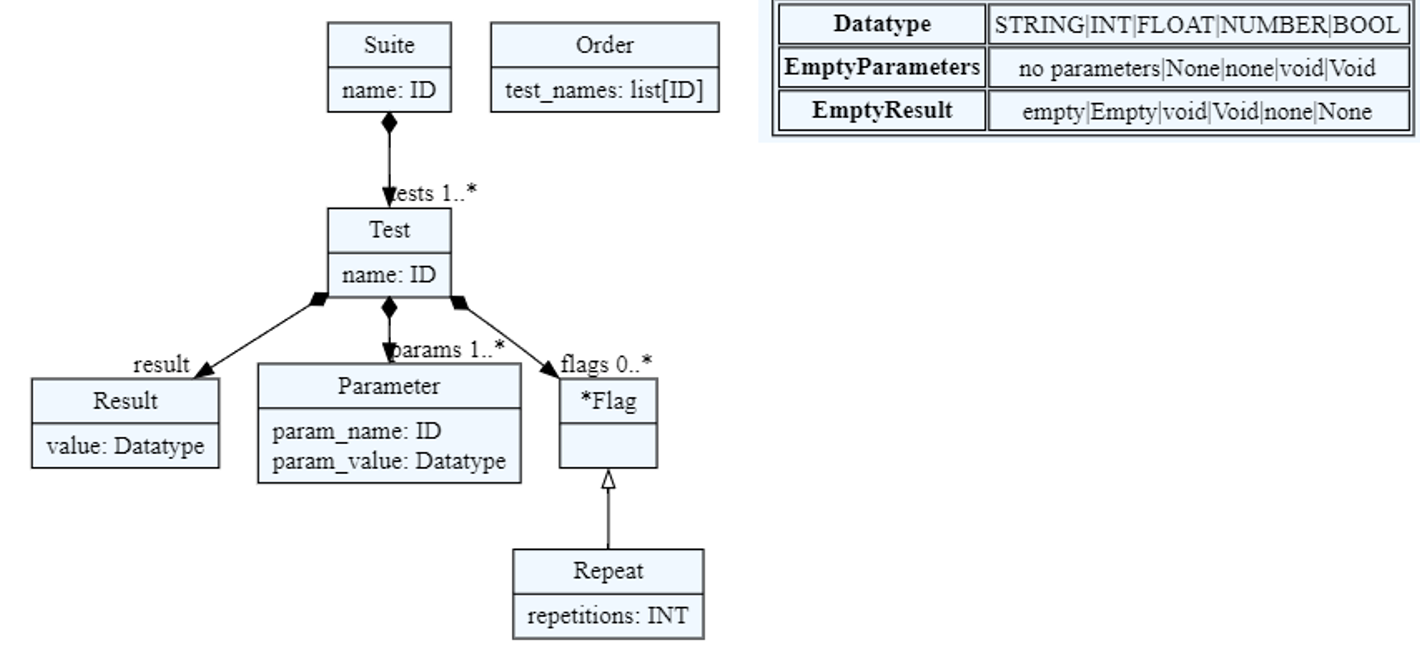
\includegraphics[width=\textwidth]{images/metamodel.png} }
\begin{center} Figure 2: Language meta-model  \end{center}

An example parse tree would be useful.

Suite mySuite

Test foo -skip -repeat 5 times
When param1=1, param2=True
Then result should be 42

The obtained parse tree from the above piece of code is constructed in Figure 3.

{ \centering 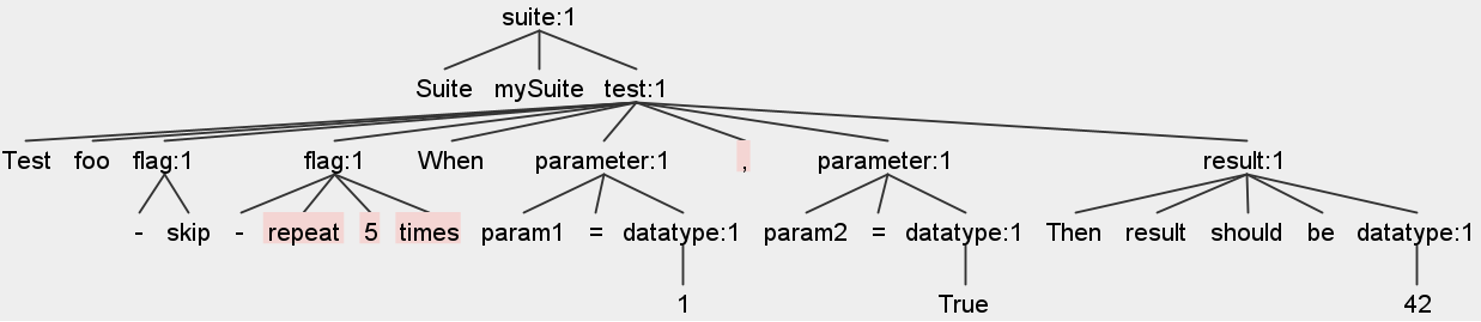
\includegraphics[width=\textwidth]{images/parse_tree.png} }
\begin{center} Figure 3: Parse Tree for example program \end{center}
